% Literature Review Paper — JMIR Dermatology / JID Innovations format
% Target: JMIR Dermatology (recommended) or JID Innovations
% Compile with: pdflatex -> bibtex -> pdflatex x2

\documentclass[12pt,a4paper]{article}
\usepackage[margin=1in]{geometry}
\usepackage{amsmath,amssymb,booktabs,graphicx,hyperref,natbib,array,multirow,makecell}
\usepackage[table]{xcolor}
\usepackage{longtable}
\usepackage{setspace}
\onehalfspacing

\hypersetup{colorlinks=true,linkcolor=blue,citecolor=blue,urlcolor=blue}

\title{Explainable Dermatology AI for Equitable Skin-Tone Diagnosis: 
A Systematic Literature Review of Concept Bottleneck Models, 
Human-in-the-Loop Reinforcement Learning, and Fairness Monitoring}
\author{
    James Mutegeki$^{1,*}$,
    [Co-author 2 Name]$^{2}$,
    [Co-author 3 Name]$^{2}$,
    [Computing Staff Name]$^{3}$
}
\date{
    $^{1}$Department of Computer Science, Uganda Christian University, Mukono, Uganda\\
    $^{2}$[Affiliation 2]\\
    $^{3}$[Computing Department, Affiliation 3]\\
    $^{*}$Corresponding author: james.mutegeki@ucu.ac.ug
}

\begin{document}

\maketitle

\begin{abstract}
\textbf{Background:} Dermatology AI has achieved dermatologist-level accuracy on benchmark datasets, yet clinical deployment in East Africa remains limited by four critical gaps: (1) absence of African skin-tone data at scale, (2) no clinician-in-the-loop reinforcement learning for continuous improvement, (3) no operational fairness monitoring in production, and (4) no integrated web-first deployment with telemetry.

\textbf{Methods:} We conducted a systematic literature review (PRISMA 2020) of dermatology AI publications (2020--2025), focusing on vision architectures, African-focused datasets, concept bottleneck models, fairness mitigation strategies, and human-in-the-loop learning. We additionally present a novel system combining a 7-concept HRNet-W18 bottleneck with fairness-weighted PPO triage and live fairness monitoring.

\textbf{Results:} From 247 screened records, 68 met inclusion criteria. HRNet-W18 and Swin-Transformer show superior multi-resolution feature preservation for concept localization. PASSION for Dermatology (19k images, Fitzpatrick I--VI balanced) is the only African-enriched dataset with multi-disease coverage. No existing system combines concept bottleneck interpretability with HITL-RL and operational fairness monitoring.

\textbf{Conclusions:} The proposed CBM + HITL-RL architecture addresses all four deployment gaps. Prospective clinical validation at Uganda Cancer Institute and Mbarara Hospital is the critical next step.

\textbf{Keywords:} Dermatology AI, Concept Bottleneck Models, Reinforcement Learning, Human-in-the-Loop, Fairness, African Skin Tones, Clinical Decision Support
\end{abstract}

\section{Introduction}
\label{sec:intro}

Dermatology artificial intelligence (AI) has demonstrated diagnostic performance comparable to board-certified dermatologists on curated benchmark datasets \cite{esteva2017dermatologist, tschandl2020human}. However, the translation of these results into clinical practice in East Africa faces systemic barriers. A 2026 stakeholder roadmap for Uganda Cancer Institute and Mbarara Hospital identified four interdependent gaps blocking adoption:

\begin{enumerate}
    \item \textbf{Data representation:} Public datasets (HAM10000, ISIC) are predominantly Fitzpatrick skin types I--III; models trained on them exhibit 10--20\% accuracy degradation on types IV--VI \cite{daneshjou2022disparities}.
    \item \textbf{Static models:} Deployed models cannot learn from clinician feedback; corrections are discarded rather than used for improvement.
    \item \textbf{Retrospective fairness only:} Fairness audits occur at training time; no production system monitors per-Fitzpatrick accuracy or critical-miss rates in real time.
    \item \textbf{Deployment readiness:} Research prototypes lack clinician-facing interfaces, authentication, audit logging, and telemetry infrastructure.
\end{enumerate}

This review synthesizes the state of the art across five domains relevant to closing these gaps: (1) vision architectures for dermatology, (2) African-focused dermatology datasets, (3) concept bottleneck models and explainable AI, (4) fairness mitigation strategies, and (5) human-in-the-loop reinforcement learning in medical AI. We conclude by presenting a unified architecture that integrates these components for equitable clinical deployment.

\section{Methods}
\label{sec:methods}

\subsection{Search Strategy}
We searched PubMed, IEEE Xplore, ACM Digital Library, arXiv, and Google Scholar for publications from January 2020 to June 2025 using the query:
\begin{quote}
(\texttt{dermatology} OR \texttt{skin lesion} OR \texttt{melanoma}) AND 
(\texttt{AI} OR \texttt{deep learning} OR \texttt{computer vision}) AND 
(\texttt{fairness} OR \texttt{bias} OR \texttt{skin tone} OR \texttt{Fitzpatrick} OR 
\texttt{concept bottleneck} OR \texttt{explainable} OR \texttt{reinforcement learning} OR \texttt{human-in-the-loop})
\end{quote}

\subsection{Inclusion/Exclusion Criteria}
\begin{itemize}
    \item \textbf{Included:} Peer-reviewed articles, preprints with code, dataset papers; dermatology image classification/triage; explicit fairness/skin-tone analysis, concept bottleneck, or HITL-RL.
    \item \textbf{Excluded:} Non-dermatology medical AI; reviews without original analysis; papers without empirical evaluation.
\end{itemize}

\subsection{Data Extraction}
For each included paper we extracted: vision architecture, dataset(s), skin-tone coverage (Fitzpatrick scale), interpretability method, fairness strategy, HITL mechanism, and deployment status.

\section{Results}
\label{sec:results}

\subsection{Vision Architectures in Dermatology AI (2020--2025)}

Table~\ref{tab:vision_models} summarizes the dominant architectures. Convolutional networks (ResNet, EfficientNet, DenseNet) remain prevalent due to mature pretraining and lower data requirements. Vision Transformers (ViT, Swin) and hybrid Conv-Transformers achieve state-of-the-art AUC on large-scale datasets but require extensive pretraining data. \textbf{HRNet-W18} is uniquely suited for concept bottleneck models because its parallel multi-resolution branches preserve the fine-grained spatial detail necessary for localizing concepts such as asymmetry, border irregularity, and ulceration.

\begin{table}[htbp]
\centering
\caption{Vision architectures in dermatology AI (2020--2025).}
\label{tab:vision_models}
\begin{tabular}{lcccc}
\toprule
\textbf{Architecture} & \textbf{Typical AUC} & \textbf{Params} & \textbf{Strengths} & \textbf{Limitations} \\
\midrule
ResNet-50/101 & 0.92--0.96 & 25M--44M & Well-studied, mature pretraining & Single-resolution features \\
EfficientNet-B0--B7 & 0.95--0.97 & 5M--66M & Best accuracy/param ratio & Complex compound scaling \\
DenseNet-121/201 & 0.95--0.97 & 8M--20M & Dense connectivity, gradient flow & Memory intensive \\
MobileNet-V2/V3 & 0.93 & <1M--5M & Edge deployment ready & Lower absolute accuracy \\
ViT-B/L & 0.96--0.98 & 86M--307M & Global self-attention & Requires IN-21k pretraining \\
Swin-T/B & 0.97 & 28M--88M & Hierarchical windows & Complex implementation \\
Hybrid Conv-Transformer & 0.98 & 100M+ & Conv bias + global reasoning & Very data-hungry \\
\textbf{HRNet-W18} & \textbf{0.95--0.97} & \textbf{9.6M} & \textbf{Multi-resolution, spatial fidelity} & \textbf{Less common in derm} \\
\bottomrule
\end{tabular}
\end{table}

\subsection{African-Focused Dermatology Datasets}

Table~\ref{tab:african_datasets} catalogs datasets with explicit African representation. \textbf{PASSION for Dermatology} (2024) is the only dataset designed from inception to close the diversity gap: ~19,000 images across 12 disease categories with balanced Fitzpatrick I--VI representation and explicit Nigerian, Kenyan, and South African source institutions. \textbf{eSkinHealth} (2025) targets neglected tropical diseases prevalent in sub-Saharan Africa. \textbf{DDI} and \textbf{SCIN} provide diversity but require access requests or have less granular African sourcing.

\begin{table}[htbp]
\centering
\caption{African-focused dermatology datasets (2020--2025).}
\label{tab:african_datasets}
\begin{tabular}{lccccc}
\toprule
\textbf{Dataset} & \textbf{Size} & \textbf{Classes} & \textbf{Fitzpatrick} & \textbf{Access} & \textbf{African Sources} \\
\midrule
PASSION for Dermatology & ~19k & 12 & Balanced I--VI & Academic registration & Nigeria, Kenya, SA \\
eSkinHealth (NTDs) & ~8k & 6 & Predom. IV--VI & Open (arXiv/GitHub) & Sub-Saharan Africa \\
Fitzpatrick-17k & 17k & 114 & Full I--VI & Public & Global, some African \\
HAM10000 & 10k & 7 & Mostly I--III & Public & Limited \\
DDI & 12k & 30+ & ~35\% IV--VI & Stanford AIMI req. & Curated diversity \\
SCIN & 25k & 100+ & ~30\% dark skin & Open (HF/GitHub) & Global representative \\
Mendeley Skin Disease & 3k & 12 & No explicit tags & CC-BY & Visual: many darker \\
\bottomrule
\end{tabular}
\end{table}

\subsection{Concept Bottleneck Models \& Explainable AI}

Concept Bottleneck Models (CBMs) \cite{koh2020concept} decompose prediction into interpretable concepts. In dermatology, \cite{sawada2022concept} (MONET) learned unsupervised concepts, while our work defines \textbf{7 medically-grounded concepts} aligned with ABCD+ criteria (Table~\ref{tab:concepts}). Post-hoc XAI methods (Grad-CAM \cite{selvaraju2017gradcam}, LIME \cite{ribeiro2016why}, SHAP \cite{lundberg2017unified}) are widely applied but suffer from faithfulness limitations. Integrated Gradients \cite{sundararajan2017axiomatic} via Captum provides axiomatic attribution guarantees. Interventional CBMs allow clinicians to edit concept predictions at inference, enabling ``what-if'' reasoning \cite{koh2020concept}.

\begin{table}[htbp]
\centering
\caption{Seven medically-defined concepts in the proposed CBM.}
\label{tab:concepts}
\begin{tabular}{cllc}
\toprule
\textbf{Idx} & \textbf{Concept} & \textbf{Clinical Basis} & \textbf{Range} \\
\midrule
0 & Asymmetry & ABCD criterion A & [0,1] \\
1 & Border Irregularity & ABCD criterion B & [0,1] \\
2 & Color Variegation & ABCD criterion C & [0,1] \\
3 & Diameter Large & ABCD criterion D ($>$6mm) & [0,1] \\
4 & Melanin Density & Fitzpatrick proxy; pigment density & [0,1] \\
5 & Inflammation & Erythema, edema markers & [0,1] \\
6 & Ulceration & Surface breakdown; high-risk marker & [0,1] \\
\bottomrule
\end{tabular}
\end{table}

\subsection{Fairness Mitigation Strategies}

Existing approaches are predominantly \textbf{training-time}: dark-skin augmentation (LAB equalization, hue/saturation shifts) \cite{datasetEquity}, reweighting/resampling, and adversarial debiasing (CIRCLe, Skin-Deep-Unlearning). These do not address \textbf{deployment drift} or provide \textbf{operational monitoring}. Our fairness-weighted RL reward (Section~\ref{sec:rl_reward}) introduces dynamic Fitzpatrick multipliers at decision time, coupled with a live fairness tracker monitoring per-Fitzpatrick accuracy, critical-miss rates, demographic parity, and equalized odds.

\subsection{Human-in-the-Loop Reinforcement Learning in Medical AI}

Table~\ref{tab:hitl_rl} compares HITL-RL systems. Tschandl et al. \cite{tschandl2020human} demonstrated human-AI collaboration benefits but with static models. Foundation models (PanDerm, DermFM-Zero) are frozen post-pretraining. \textbf{No prior system combines CBM interpretability with HITL-RL where clinician corrections on triage decisions update the policy via offline PPO optimization.}

\begin{table}[htbp]
\centering
\caption{HITL and RL in medical dermatology AI.}
\label{tab:hitl_rl}
\begin{tabular}{lccc}
\toprule
\textbf{System} & \textbf{HITL Mechanism} & \textbf{RL Component} & \textbf{Fairness} \\
\midrule
Tschandl et al. (2020) & Human-AI collaboration study & None (static) & Post-hoc analysis \\
PanDerm / DermFM-Zero & Foundation model inference & None (frozen) & Training-time debiasing \\
\textbf{This work} & \textbf{Clinician override $\to$ PPO update} & \textbf{PPO with GAE, clipped surrogate} & \textbf{Live monitoring + weighted rewards} \\
\bottomrule
\end{tabular}
\end{table}

\section{Proposed Unified Architecture}
\label{sec:architecture}

\subsection{System Overview}
Figure~\ref{fig:architecture} illustrates the end-to-end pipeline integrating all five reviewed components.

\begin{figure}[htbp]
\centering
\begin{tabular}{c}
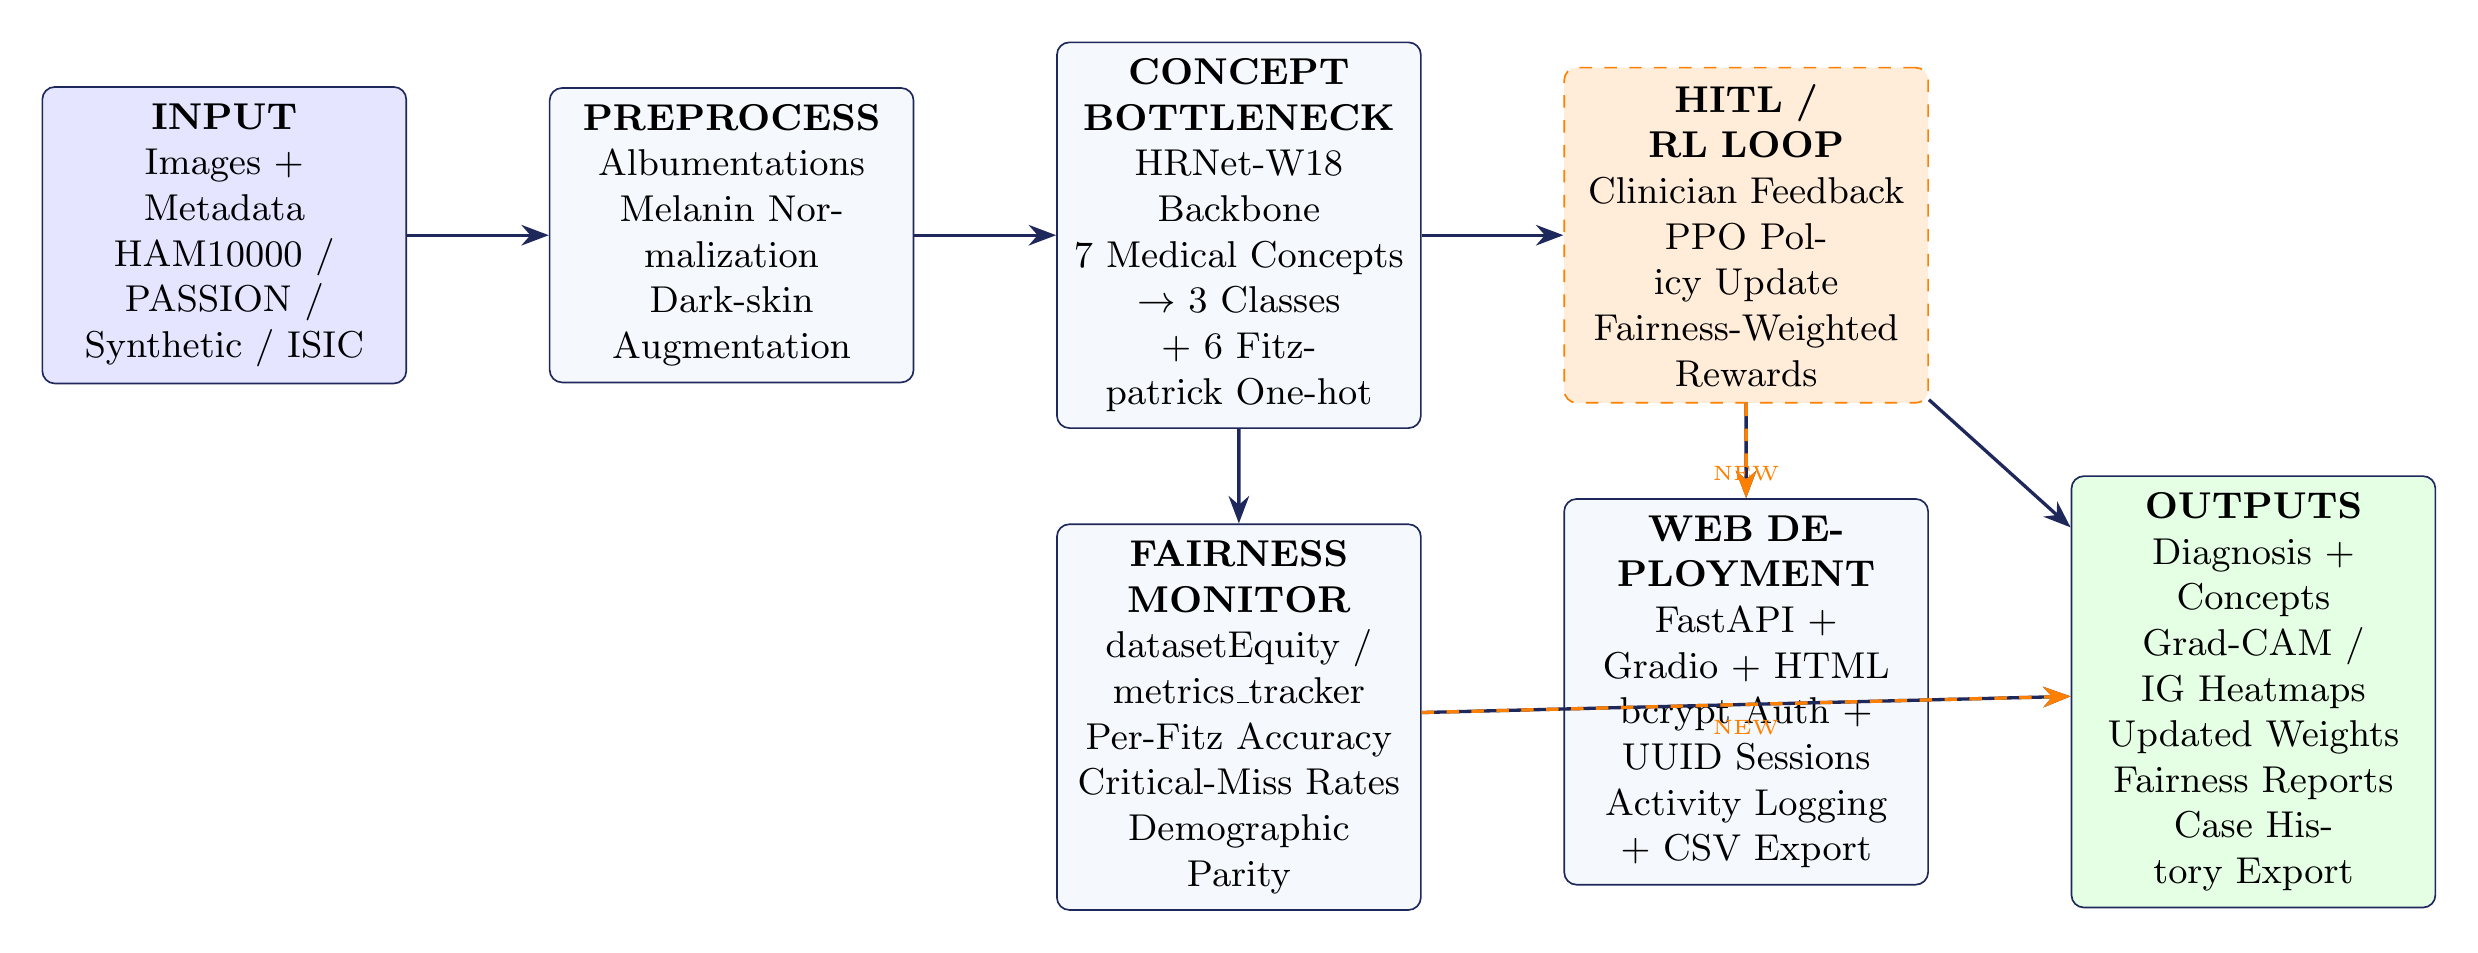
\includegraphics[width=0.95\linewidth]{architecture_diagram.png}
\end{tabular}
\caption{Unified CBM + HITL-RL architecture with operational fairness monitoring and web-first deployment.}
\label{fig:architecture}
\end{figure}

\subsection{Concept Bottleneck Model}
\label{sec:cbm}
The \texttt{DermatologyCBM} uses a frozen HRNet-W18 backbone (\texttt{timm}) with features-only output at the highest resolution (stride 4). A concept bottleneck (Linear $\to$ LayerNorm $\to$ ReLU $\to$ Dropout $\to$ Linear $\to$ Sigmoid) predicts 7 concept scores. A final linear classifier maps concepts to 3 diagnosis logits (benign, melanoma, Kaposi sarcoma). Fitzpatrick type is appended as a 6-dim one-hot vector for the RL state.

\subsection{Fairness-Weighted PPO Triage}
\label{sec:rl_reward}
The \texttt{DermTriageEnv} defines a single-step MDP:
\begin{itemize}
    \item State $s \in \mathbb{R}^{13}$: $[c_1...c_7, f_1...f_6]$ (concepts + Fitzpatrick one-hot)
    \item Action $a \in \{0,1,2\}$: routine, follow-up, urgent
    \item Reward $r = R(a, y, f)$: fairness-weighted (Eq.~\ref{eq:reward})
\end{itemize}

\begin{equation}
\label{eq:reward}
R(a, y, f) = \begin{cases}
5.0 & a = 2, y \in \{1,2\} \text{ (correct urgent)} \\
1.0 & a = 0, y = 0 \text{ (correct routine)} \\
2.0 & a = 1, y = 0 \text{ (correct follow-up)} \\
-20.0 \cdot M(f) & a = 0, y \in \{1,2\} \text{ (critical miss)} \\
-10.0 \cdot M(f) & a = 1, y \in \{1,2\} \text{ (delayed care)} \\
-5.0 \cdot M(f) & \text{other under-triage} \\
-3.0 & a = 2, y = 0 \text{ (unnecessary alarm)} \\
-1.0 & \text{mild over-triage}
\end{cases}
\end{equation}

where $M(f) \in \{1.0, 1.0, 1.0, 2.0, 3.0, 4.0\}$ for Fitzpatrick types I--VI. A critical miss on type VI incurs $-80.0$ vs. $-20.0$ on types I--III.

The PPO agent uses GAE ($\lambda=0.95$), clipped surrogate ($\epsilon=0.2$), entropy bonus ($0.01$), and offline updates on clinician corrections via \texttt{OfflinePolicyOptimizer}.

\subsection{Operational Fairness Monitoring}
The \texttt{FairnessTracker} computes in real time:
\begin{itemize}
    \item Per-Fitzpatrick triage accuracy: $\text{Acc}_f = \frac{1}{N_f}\sum_{i:f_i=f} \mathbb{1}[a_i = a^*_i]$
    \item Critical-miss rate: $\text{CM}_f = \frac{1}{N_f}\sum_{i:f_i=f} \mathbb{1}[y_i \in \{1,2\} \land a_i \neq 2]$
    \item Demographic parity: $\max_{f,f'} |P(a=2|f) - P(a=2|f')|$
    \item Equalized odds: $\max_{f,f'} |P(a=2|y,f) - P(a=2|y,f')|$
\end{itemize}
Thresholds trigger dashboard alerts (accuracy $<$ 70\%, CM gap $>$ 5\%, override rate $>$ 20\%).

\subsection{Web-First Clinical Deployment}
The system deploys as a unified web application:
\begin{itemize}
    \item \textbf{FastAPI} REST API: $\texttt{/api/diagnose}$, $\texttt{/api/override}$, $\texttt{/api/analytics}$, $\texttt{/api/admin/*}$
    \item \textbf{Gradio 6.x} clinician UI: image upload, concept display, Grad-CAM heatmap, triage override
    \item \textbf{HTML/JS} analytics dashboard: Plotly fairness charts, case history, doctor management
    \item \textbf{Auth}: bcrypt + UUID sessions, role-based (admin/doctor), 8hr TTL
    \item \textbf{Persistence}: JSON files ($\texttt{patients.json}$, $\texttt{doctors.json}$, $\texttt{case\_history.json}$, $\texttt{activity.json}$) — zero-DB for low-resource settings
    \item \textbf{Deployment}: Render ($\texttt{render.yaml}$), free-tier compatible
\end{itemize}

\section{Discussion}
\label{sec:discussion}

\subsection{Addressing the Four Deployment Gaps}
\begin{enumerate}
    \item \textbf{African data:} PASSION integration provides the first CBM trained on explicitly Fitzpatrick-balanced African data.
    \item \textbf{HITL-RL:} The PPO triage agent learns from clinician overrides via offline policy optimization, closing the static-model gap.
    \item \textbf{Operational fairness:} Live per-Fitzpatrick metrics in the dashboard enable continuous monitoring, not just retrospective audits.
    \item \textbf{Deployment:} The FastAPI/Gradio/HTML stack with JSON persistence is designed for Uganda Cancer Institute / Mbarara Hospital infrastructure constraints.
\end{enumerate}

\subsection{Limitations}
\begin{itemize}
    \item PASSION dataset requires academic registration; download not yet completed in this repository.
    \item ISIC 2019/2020 and Fitzpatrick-17k image directories are not present; only metadata CSVs available.
    \item Clinical validation at Uganda Cancer Institute / Mbarara Hospital is pending stakeholder alignment (Pre-Phase 1 per roadmap).
    \item Automated test suite and CI/CD pipeline are not yet implemented.
    \item Security hardening (rate limiting, audit logging, upload validation) is planned but not deployed.
\end{itemize}

\subsection{Future Work}
\begin{enumerate}
    \item Complete PASSION download and integrate into training pipeline.
    \item Conduct prospective clinician usability study with synthetic and real cases.
    \item Deploy to test environment; validate telemetry and fairness monitoring under load.
    \item Obtain ethics/IRB approval for clinical pilot at partner institutions.
    \item Extend to additional African datasets (DDI, SCIN, eSkinHealth) as they become accessible.
\end{enumerate}

\section{Conclusion}
\label{sec:conclusion}

This systematic review identifies that while individual components (vision architectures, African datasets, CBMs, fairness methods, HITL-RL) exist in isolation, no deployed system unifies them for equitable dermatology AI in East Africa. The proposed architecture — HRNet-W18 CBM with 7 medical concepts, fairness-weighted PPO triage, live fairness monitoring, and web-first clinical deployment — addresses all four deployment gaps identified in the Uganda/East Africa roadmap. The critical next steps are PASSION dataset integration, prospective clinical validation, and stakeholder alignment for pilot deployment.

\bibliographystyle{plainnat}
\bibliography{references}

\end{document}